%%%%%%%%%%%%%%%%%%%%%%%%%%%%%%%%%%%%%%%%%
% Uppsala University Assignment Title Page 
% LaTeX Template
% Version 1.0 (27/12/12)
%
% This template has been downloaded from:
% http://www.LaTeXTemplates.com
%
% Original author:
% WikiBooks (http://en.wikibooks.org/wiki/LaTeX/Title_Creation)
% Modified by Elsa Slattegard to fit Uppsala university
% License:
% CC BY-NC-SA 3.0 (http://creativecommons.org/licenses/by-nc-sa/3.0/)

%\title{Title page with logo}
%----------------------------------------------------------------------------------------
%	PACKAGES AND OTHER DOCUMENT CONFIGURATIONS
%----------------------------------------------------------------------------------------

\documentclass[12pt]{article}
\usepackage[T1]{fontenc}
\usepackage[swedish]{babel}
\usepackage[utf8]{inputenc}
\usepackage{amsmath}
\usepackage{graphicx}
\usepackage{float}
\usepackage[hidelinks]{hyperref}
\usepackage[all]{hypcap}

\begin{document}

\begin{titlepage}

\newcommand{\HRule}{\rule{\linewidth}{0.5mm}} % Defines a new command for the horizontal lines,
change thickness here

\center%% change thickness here

\center% Center everything on the page
 
%----------------------------------------------------------------------------------------
%	HEADING SECTIONS
%----------------------------------------------------------------------------------------

\textsc{\LARGE Uppsala University}\\[1.5cm] % Name of your university/college

\includegraphics[scale=.1]{Uppsala_University_seal_svg.png}\\[1cm] % Include a department/university logo - this will require the graphicx package
\textsc{\Large Introduktion till informationsteknologi}\\[0.5cm] % Major heading such as course name
%----------------------------------------------------------------------------------------
%	TITLE SECTION
%----------------------------------------------------------------------------------------

\HRule\\[0.4cm]
{ \huge \bfseries A Bug's Life}\\[0.4cm] % Title of your document
\HRule\\[1.5cm]
 
%----------------------------------------------------------------------------------------
%	AUTHOR SECTION
%----------------------------------------------------------------------------------------

\begin{minipage}{0.6\textwidth}
\begin{flushleft} \large
\emph{Authors:}\\
Anonymous \textsc{Student Team}\\ % Your name
Aletta \textsc{Nylén}\\ % Your name
\end{flushleft}

\end{minipage}\\[2cm]

% If you don't want a supervisor,
% uncomment the two lines below and remove the section above
%\Large \emph{Author:}\\
%John \textsc{Smith}\\[3cm] % Your name

%----------------------------------------------------------------------------------------
%	DATE SECTION
%----------------------------------------------------------------------------------------

{\large \today}\\[2cm] % Date,
% change the \today to a set date if you want to be precise

\vfill % Fill the rest of the page with whitespace


% TODO: Related work
% Swarm intelligence har fått relevans inom datavetenskapen vid lösning av shortest path och travelling salesmanproblemet~\cite{dorigo1997ant}.



\end{titlepage}
\tableofcontents
\newpage
\section{Inledning}
\textit{Swarm intelligence} är ett koncept som innebär att en grupp av organismer,
helt utan en ledare i centrum och endast med begränsad individuell intelligens, 
i grupp kan lösa komplexa problem.
Till exempel består ett försvar av soldater.
Varje soldat kan inte göra så mycket själv, men som grupp är soldaterna mycket starkare.
Något annat man kan göra är att simulera idrottslag.
Till exempel kan man simulera hur fotbollsspelare borde röra sig på en spelplan för att hjälpa varandra och få ut mer av sitt spel.
Med avancerade varianter av swarm intelligence kan man räkna ut hur man optimalt kan röra sig för att få så stort övertag som möjligt.
Genom att simulera enklare varianter av swarm intelligence kan man dra lärdomar som senare kan användas för att simulera mer komplicerade varianter.

BugsLife är en simulering där myror kan hitta utplacerad mat och sedan ta tillbaka den till sitt bo.
Genom att lämna feromoner på vägen kan myrorna sedan hitta tillbaka till maten genom att följa sina egna spår.
Systemet är konstruerat så att det är fullständigt concurrent och arbetar helt utan någon supervisor eller tidssynkronisering.
Detta har åstadkommits genom att låta varje objekt i simuleringen vara en egen process där all kommunikation mellan processerna sker via meddelandeöverföring.
Dessutom använder systemet sig av actor-modellen och är fritt från deadlocks.

\section{Relaterat arbete}
~\cite{dorigo1997ant}

\section{Översikt över systemet}
Användaren startar simuleringen utan input-parametrar och systemet körs sedan automatiskt och kräver ingen interaktion från användaren.
Vid första anblick kan myrkolonin uppfattas som enkel,
men komplexiteten i simuleringen ligger i systemarkitekturen och de algoritmer myrorna använder sig av för att effektivisera hämtningen av mat.
En skärmdump av simuleringen kan ses i Figur~\ref{fig:screen-dump}.

\begin{figure}[H]
    \centering
    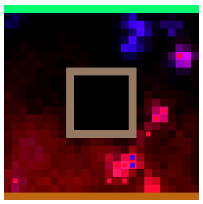
\includegraphics[width=0.5\textwidth]{BugsLife-Fig1.png}
    \caption{
        En skärmdump av simuleringen.
        De brun/orangea rutorna är myrbo,
        de gröna är mat,
        de bruna/gråa är väggar.
        De små röda rutorna är myror som letar efter mat och de små blåa rutorna är myror som är på väg hem med mat.
        I bakgrunden syns feromonerna.
    }\label{fig:screen-dump}
\end{figure}

\subsection{Concurrency}
På grund av den höga nivån av autonomitet kombinerat med separationen mellan de olika processerna används så kallad eventdriven programmering.
Eventdriven programmering är när ett program styrs av externa händelser som inte går att kontrollera eller förutse.
Ett exempel på det är vid programmering av användargränssnitt,
då det inte går att förutspå när eller i vilken ordning användaren kommer att ge input till systemet.

Systemet använder sig av actor-modellen då den ger bra möjligheter att på ett konceptuellt och effektivt sätt implementera eventdriven programmering då den ger en möjlighet att fokusera på en modul i taget utan att behöva ta hänsyn till hur de andra modulerna är implementerade.
Det enda som behövs är ett meddelandeprotokoll som alla moduler följer.

Det är viktigt att påpeka att systemet använder sig av asynkron eventdriven programmering.
Detta ger upphov till många problem då det inte går att garantera att meddelandena kommer i rätt ordning.
Problemen löses med hjälp av meddelandefiltrering,
som innebär att en process väntar på ett specifikt meddelande innan den går vidare och buffrar de meddelanden som kvarstår.
Varje process behöver då ha ett speciellt tillstånd när den accepterar alla nya förfrågningar.

\subsection{Systemdesign}
I figur~\ref{fig:sysark-overview} syns en schematisk överblick av systemarkitekturen.
Alla moduler arbetar helt asynkront och all kommunikation mellan modulerna sker via meddelanden.

\begin{figure}[H]
    \centering
    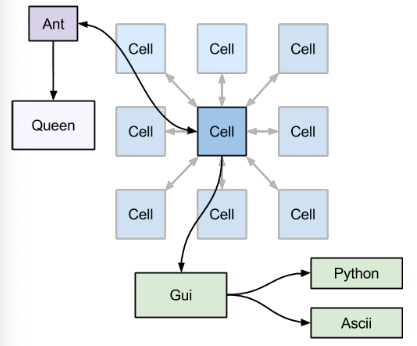
\includegraphics[width=\textwidth]{BugsLife-Fig2.png}
    \caption{En schematisk överblick över systemarkitekturen}\label{fig:sysark-overview}
\end{figure}

\subsubsection{Ant}
Ant-modulen är den modul som implementerar myran.
Ant-modulen innehåller de funktioner som krävs för att myran skall kunna fatta beslut över hur den ska agera baserat på hur dess omgivning ser ut.
Detta gör den genom att skicka förfrågningar till den cell myran befinner sig på och sedan använda svaret för att autonomt fatta ett beslut om vilken handling som är lämpligast.
Under normal drift så tar myran aldrig emot några förfrågningar från någon annan process,
endast svar från den cell som den befinner sig i.

Ant-modulen är utrustad med funktionalitet så att myran kan analysera den information som ges av grannskapet till cellen den står i.
Informationen gör det möjligt för myran att fatta ett beslut,
baserat på vad myrans omgivning består av.
Myror i det verkliga livet kommunicerar med varandra genom olika typer av feromoner,
detta för att meddela var maten finns.
Det är viktigt att myrorna kan inspektera sin omgivning så att den kan fatta ett beslut baserat på vad andra myror har upptäckt i omgivningen.
Finns det feromoner som indikerar till myran att det finns föda i närheten kan myran ta ett beslut att röra sig i den riktningen och leta rätt på födan.
Myrorna använder sig även av feromoner för att hitta hem till sitt näste.

\subsubsection{Cell}
Cell-modulen representerar cellerna där varje cell är en ruta i det rutnät som utgör världen där myrorna lever.
Cellen är det objekt som innehåller den relevanta informationen för systemet.
En cell innehåller information om vad det är för typ av cell,
om cellen exempelvis representerar ett myrbo, 
om det finns mat på cellen,
om det står en myra på cellen 
samt intensiteten för dem olika feromonerna på cellen.
Förutom att lagra information hanterar cellen också meddelanden.
Cellen tar emot och besvarar förfrågningar från myran som står på cellen, tar emot, besvara och skickar förfrågningar till cellerna i dess direkta grannskap samt skickar meddelanden till GUI-modulen.
Den enda gång en cell kan skicka förfrågningar till en annan cell är om cellen fått en förfrågan att skicka en förfrågan.

\subsubsection{Message\_Buffer}
Message Buffer är den modul som hanterar kommunikationen av meddelanden mellan processerna.
Modulen exporterar receiver-funktionen som är central för att använda den typ av eventdriven programmering som används.
Receiver-funktionen används för att hantera deadlocks och filtrering av meddelandekön.

\subsubsection{GUI}
GUI-modulen är implementerad i Python och Erlang med hjälp av ErlPort.
Modulen tar emot och behandlar meddelanden innehållandes cellernas tillstånd från cellerna.
Informationen omvandlas till Pythons syntax via Erlport och skickas till en Python-instans som hanterar den grafiska representationen.

\subsubsection{Grid\_Init}
Modulen används för att bygga upp världen samt placera alla celler och länka ihop dessa.
Grid Init modulen tilldelar även alla celler dess initiala attributer samt skapar,
placerar och startar alla myrorna. Grid init initierar även en Queen-process.
Myrorna skickar statistik till Queen-processen,
som används för debugging och prestandamätning.

\section{Implementation}\label{sec:implementation}
Systemet implementerades i Erlang då det är ett väletablerat och stabilt språk som är byggt kring actor-modellen och meddelandeöverföring.
Utöver Erlang används Python för den grafiska delen och ErlPort~\cite{erlport} för kommunikationen mellan Erlang och Python.
Implementationen av ErlPort har fungerat mycket bra och har gett oss ett smidigt interface mellan Erlang och Python.

\subsection{GUI}
GUI-modulen initieras med att skapa en lista motsvarande hela griden,
den fylls med tomma atomer som Python-modulen inte ritar ut.
GUI-modulen körs i en main loop som tar emot meddelanden från cell-modulerna,
bearbetar dessa och fyller på den initierade listan.

En algoritm används för att fördela listan på rätt X och Y koordinater,
koordinaterna är angivna i meddelandet från cellen.
Listan skickas via ErlPort till Python där den ritas upp grafiskt.

\subsubsection{Erlport}
Erlport är ett bibliotek som gör det möjligt för Erlang att kommunicera med andra programmeringsspråk.
I dagsläget har Erlport stöd för Python och Ruby.

För att Erlport ska kunna kommunicera med Python så skapas först en Python-instans.
En Python-instans är i princip en OS-process som representeras i Erlang av en Erlang process.
Man kan skicka och ta emot medelanden mellan Erlang och Python på samma sätt som man skickar meddelanden mellan vanliga processer i Erlang.

\subsubsection{Pygame}
För den grafiska renderingen i projektet används det community-utvecklade Pythonbiblioteket Pygame.
Pygame är ett bibliotek av färdigutvecklade moduler till Python designade för att enkelt kunna skapa spel med en enkel grafisk implementation.
Pygames design gör att det är enkelt att använda på alla plattformar som har stöd för Python.

\subsection{Ants and Cells}
Ant-modulen och Cell-modulen är väldigt lika varandra i sin implementation.
Båda modulerna består av en initialiseringsfunktion som används för att starta processer.
Funktionen inväntar de meddelanden som är nödvändiga för att starta processerna.
Detta kan till exempel vara ett meddelande om att myran har placerats korrekt och att cellerna har fått sitt grannskap definierat.

Cellerna och myrorna går efter ett meddelande till sin mainfunktion där de inväntar nya förfrågningar.
Om det inte finns några obehandlade meddelanden kommer myrorna att agera spontant.
När cellerna och myrorna får ett inkommande meddelande kommer de att anropa en funktion specifikt för den typen av meddelande.
Dessa funktioner kan skicka och ta emot meddelanden själva med hjälp av meddelandefiltreringen.
När en förfrågan eller annat meddelande har behandlats kommer processen återgå till sin mainfunktion.
Om ett felaktigt eller otillåtet meddelande inkommer under någon del av exekveringen så kommer hela systemet att krascha.

Cellerna kommer vid varje inkommen förfrågan,
beroende av cellens tillstånd,
automatiskt genomföra en uppdatering av dess feromonnivåer.
Detta sker som en funktion av den faktiska tiden (wall-time) som har gått sedan cellen senast uppdaterades.

Om en cell har attributet block så kan en myra inte gå dit och alla \texttt{place\_ant} förfrågningar kommer att misslyckas.

\subsubsection{Myrans algoritm}
Myran beslut baseras på en väldigt enkel algoritm.
Myran kan vara i två olika tillstånd \texttt{searching\_for\_food} och \texttt{returning\_with\_food}.

När myran letar efter mat så kommer den att undersöka cellen den står i,
om det finns mat i cellen så kommer myran att försöka plocka upp maten.
Om myran lyckas plocka upp mat kommer den att byta tillstånd till \texttt{returning\_with\_food},
om myran misslyckas med att plocka upp mat så kommer den att fortsätta leta efter mat i andra celler.

När myran letar efter mat så kommer den att be cellen den står i att skicka tillbaka information om alla celler i dess grannskap.
Myran kommer sedan att studera sitt grannskap och sortera cellerna efter hur mycket \texttt{food\_feremone} varje cell innehåller och sedan genom \textit{rank-selection} att välja den riktingen den skall gå i.
Rank-selection innebär att den med en förutbestämd sannolikhet \textit{p} kommer att gå till den cellen med det högsta antalet feromoner.
Om den inte väljer den riktningen så kommer den att gå till den cellen med näst högst riktning med samma sannolikhet \textit{p}.

Myran kommer efter varje genomförd förflyttning att släppa feromoner på den cellen där den tidigare var.
Då myran letar efter mat kommer den att släppa \texttt{base\_feremone} och då den går tillbaka med maten så kommer den att släppa \texttt{food\_feremone}.

Då myran går tillbaka med mat så kommer den att följa en snarlik algoritm men istället leta efter den högsta koncentrationen av \texttt{base\_feremone}.

I figur~\ref{fig:ant-algorithm} finns en flow-chart om hur algoritmen ser ut.


\begin{figure}[H]
    \centering
    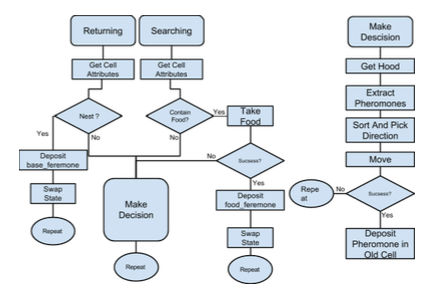
\includegraphics[width=\textwidth]{BugsLife-Fig3.png}
    \caption{Flowchart över myrans algoritm}\label{fig:ant-algorithm}
\end{figure}
\newpage

\subsubsection{Grid\_Init}
Grid init är den modul som bygger upp världen.
Det första som den modulen gör är att den startar alla cell-processer.
Det krävs att GUI-modulen är startad,
dess PID kommer att skickas med till alla celler.
Den kommer sedan att skicka ut \texttt{set\_cell\_attribute} medelanden till alla dessa celler med cellernas attribut.
Grid\_init kommer sedan att initiera en \textit{Queen}\footnote{Queen processen samlar in statistik från myrorna och används endast för debugging och testning.} process och starta alla myror och försöka placera ut dem på de celler där de skall starta.
När alla myror har blivit utplacerade så kommer Grid\_init modulen att skicka \texttt{start\_ant} medelanden till myrorna vilket kommer att starta simuleringen.

\subsection{Concurrency}
Då concurrencyn i systemet uteslutande bygger på actor-modellen och message passing så har systemet tre definierade klasser av meddelanden.

\begin{itemize}
    \item Enkelrikatade meddelanden på formen \\
    \texttt{\{Pid,\{Type,Payload\}\}} eller \texttt{\{Pid,Type\}} \\
    Enkelriktade meddelanden är meddelanden som inte kommer att resultera i att något svar inkommer.
    \item Förfrågningar på formen \\
    \texttt{\{Pid,Reference,Payload\}} \\
    Alla förfrågningar resulterar i att processen blockerar och inväntar svarsmeddelanden.
    \item Svarsmeddelanden på formen \\
    \texttt{\{Pid,Reference,Request\_Reference,\{Type,Reply\_Payload\}\}} \\
    Svar är de meddelanden som skickas som svar på förfrågningar.
\end{itemize}

För alla meddelanden gäller att \texttt{Pid} är process id:t hos den process som skickar meddelandet,
\texttt{Payload} är vad meddelandet faktiskt innehåller och \texttt{Reference} är en referens som den skickande processen ger meddelandet.
\texttt{Request\_Reference} är en referens från en förfrågning till vilket detta är ett svar.

Då systemet faller under \textit{asynkron eventdriven programmering} så kan vissa problem uppstå om vi inte är försiktiga med hur vi implementerar systemet.
Det naiva tillvägagångssättet hade varit en så kallad \textit{Fifo, run to completion} metod.
Detta innebär att man accepterar varje meddelande, hanterar det och låter det köra tills det att det är klart innan man hanterar nästa meddelande.
Fifo-metoden leder dock till problem med att man måste hålla explicit koll på vilket tillstånd processen är i och ha en plan för hur man ska hantera alla kombinationer av meddelande-tillstånd.
Detta skulle ha lett till extremt komplicerad och svårhanterlig kod.~\cite{wiger-complexity}

Lösningen på detta är att använda vad vi kallar för \textit{state-driven message handling},
vilket är att vi låter en process tillstånd diktera vilka meddelanden som den kommer att hantera.
Det vi gör är att vi implementerar ett meddelandefilter som bara returnerar rätt meddelande (baserat på meddelandets unika tag/referens) och alla andra meddelanden som inkommer läggs på en buffer så att de senare kan hanteras.

Detta leder till att koden blir kortare och lättare att underhålla då vi på ett lätt sätt kan hantera hur systemet beter sig.
Det finns dock ett krav på att alla processer måste ha ett eller flera tillstånd då de accepterar nya meddelanden.
I detta tillstånd kommer meddelanden som ligger på buffern att hanteras först och när buffern är tom kommer de nya meddelandena att hanteras.

\subsubsection{Deadlocks}
Simuleringen är full av deadlocks och de uppstår ofta.
Därför behövs ett system för att upptäcka och lösa dessa.

För enklare deadlocks går detta att lösa effektivt och deterministiskt.
Om en process väntar på svar på en förfrågan så kommer den att blockera.
Om en process väntar på ett svar från en annan process men får en förfrågan från den processen innan den har fått svar så har ett deadlock uppstått.
Processen som upptäcker att ett deadlock har uppstått kommer direkt att ge svar om misslyckande till den förfrågan som orsakade deadlocken.
Det leder till att den andra processen kommer sluta blockera och förfrågan kan därefter hanteras.
Detta förutsätter att det alltid är tillåtet för en förfrågan att misslyckas och att en process alltid kommer efter en finit tid kunna hantera nya förfrågningar efter det att en förfrågan har misslyckats.

Den här metoden kan bara endast lösa deadlocks som uppstår mellan två processer,
men systemet drabbas ständigt av mer komplicerade deadlocks.

För att lösa mer komplicerade distribuerade deadlocks skapades en metod som är väldigt simpel men mycket effektiv.
Metoden löser alla deadlocks helt automtiskt och kräver inte att några rollbacks måste genomföras eller analys av det globala tillståndet med en Wait-For-graf.~\cite{krzyzanowski-ddeadlock}
Metod kräver inte heller att några probe meddelanden skickas mellan processerana som i Chandy-Misra-Haas algoritmen.~\cite{chandy1983distributed}

Dock så predikeras vår metod på en uppsättning krav på systemet.

\begin{itemize}
    \item Alla förfrågningar kan misslyckas på ett väldefinierat sätt.
    \item Alla processer kommer att invänta ett svar efter en förfrågan har skickats.
    \item Från det att ett svar på en förfrågan har inkommit kommer processen alltid att inom en finit tid drivas till ett tillstånd där den accepterar inkommande förfrågningar.
\end{itemize}

Dessa är en uppsättning preliminära predikat.
Det kan finnas ytterligare begränsningar som har missats då de inte är applicerbara på vårt system.
Aven då dessa predikat
kan förefalla vara hårda så innebär inte det att funktionaliteten drabbas signifikant.
De tillåter att en process som väntar på ett svar fortfarande kan hantera vissa meddelanden och skicka nya förfrågningar till processer.
De tillåter även att man implementerar en prioritering av olika typer av förfrågningar eller olika typer av processer.

När en process väntar på svar från en annan process så kommer den att efter en viss förutbestämd tid (timeout),
skicka automatiska fail-svar till alla inkomna förfrågningar som ligger på dess meddelande-buffer.
Detta kommer att repeteras tills att ett svar har inkommit.
Ni kan se en schematisk beskrivning av algoritmen i figur~\ref{fig:deadlock}.

\begin{figure}[H]
    \centering
    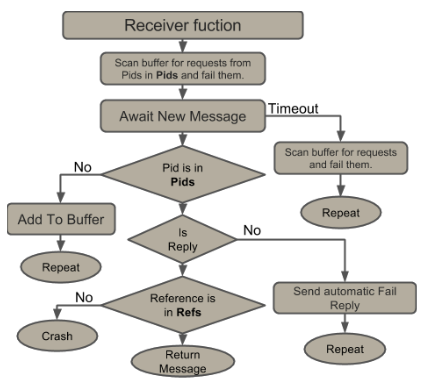
\includegraphics[width=\textwidth]{BugsLife-Fig4.png}
    \caption{
        En schematisk överblick över hur meddelandefiltreringen och deadlockhanteringen fungerar.
        \textbf{Refs} är en lista med de referenser från de förfrågningar meddelanden som har skickats.
        \textbf{Pids} är en lista med de Pids som förfrågningarna har skickats till.
    }\label{fig:deadlock}
\end{figure}

Vår metod har dock den nackdelen att den ofta kommer att upptäcka falska deadlocks,
det vill säga att den kommer att tro att det finns ett deadlock när det inte gör det och i onödan avvisa vissa förfrågningar.
Detta leder till att \textbf{Timeout} parametern måste finjusteras.
En timeout som är för lång kommer innebära att deadlocks kommer att ligga kvar för länge innan de upptäcks och delar av simuleringen kommer att lagga.
En för kort timeout kommer att leda till att väldigt många förfrågningar kommer att avisas i onödan vilket också kan påverka systemets prestanda.

\section{Slutsatser}
Vi har lyckats göra en representation av en myrkoloni som samlar mat och kommunicerar med varandra med hjälp av feromoner.
Myrorna kan även undvika olika hinder och objekt.
Aven om vi inte riktigt lyckades implementera allt vi hade iåtanke när projektet började så är vi nöjda med slutresultatet.
Det är svårt att få en verklig uppfattning av problemen och utmaningarna med ett arbete innan man satt igång med grunden på vilken andra implementationer ska vila.
Vi bestämde oss för att se till att göra en grundläggande representation av en myrkoloni och se till att denna har god concurrency och en felfri körning,
detta har vi uppnåt och även utvecklat en grafisk representation Det är detta som vi nämnde tidigare, som är vår grund.
På denna grund kan man enkelt bygga ut och genom detta implementera flera funktioner,
som till exempel flera olika typer av mat, fientliga insekter och en konkurrerande myrkoloni.
Aven om vår första tanke var att använda det nya och lite mer spännande språket Nim,
adie.

\bibliographystyle{ieeetr}
\bibliography{refs}
\end{document}